\chapter{SYSTEM DESIGN AND IMPLEMENTATION }
\patchcmd{\chapter}{\thispagestyle{fancy}}{}{}
\hrulefill\\
\thispagestyle{empty}

\section{Existing System}
{%\noindent
Traditional resume screening systems mainly rely on manual processes where recruiters read and evaluate resumes individually. This approach is time-consuming and inefficient, especially when organizations receive thousands of applications for a single job role. Due to time constraints, recruiters may not thoroughly evaluate each resume, leading to inconsistent hiring decisions and potential loss of talented candidates.}


\vspace{6pt}
{%\noindent 
With the introduction of Applicant Tracking Systems (ATS), the process became partially automated. These systems filter resumes based on keywords, predefined rules, and formatting patterns. However, they primarily depend on exact keyword matching and lack the ability to understand context or semantics. As a result, candidates with relevant skills.}


\vspace{6pt}
{%\noindent 
Existing systems also struggle with unstructured data, as resumes come in various formats such as PDFs, Word files, and creative templates. Many ATS tools fail to properly parse resumes with complex layouts, tables, or graphics, leading to incorrect data extraction or rejection of valid applications.}

\vspace{6pt}
{%\noindent 
Additionally, traditional systems lack transparency and feedback mechanisms. Candidates are often not informed why their resumes were rejected, making it difficult for them to improve. The absence of intelligent analysis and explanation reduces trust in automated recruitment systems.}

[Resume Upload] → [Keyword Matching] → [Basic Filtering] → [Shortlisting]

\begin{figure}[ht]
\centering
 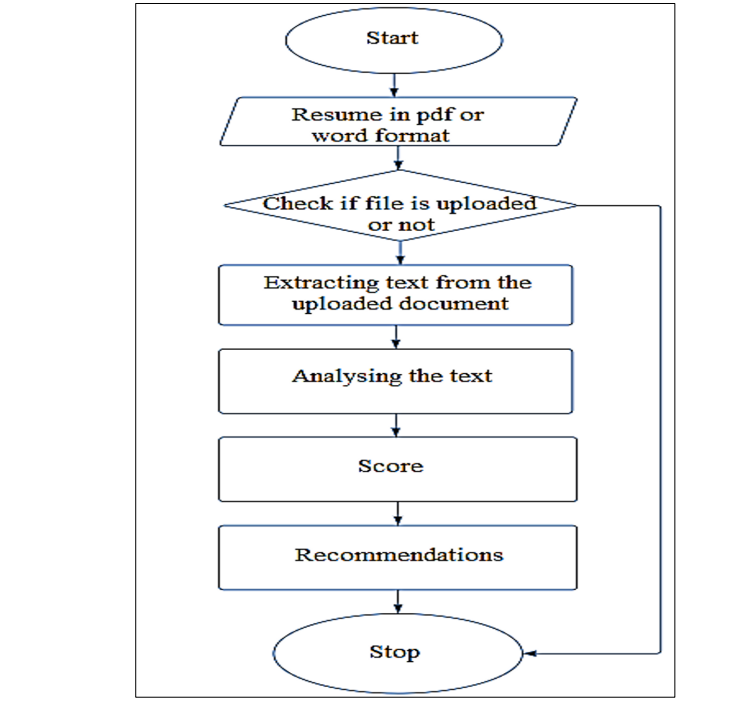
\includegraphics[width=0.6\textwidth]{images/Existing System .png}
 \captionof{figure}{Existing system}
\end{figure}

\section{Limitations of Existing Architecture}


One major limitation of existing systems is their heavy reliance on keyword matching. These systems fail to capture semantic meaning and contextual relationships between words, which can result in rejecting qualified candidates who use different terminology to describe their skills.

\vspace{6pt}
{%\noindent 
Another limitation is bias in decision-making. Manual screening introduces human bias, while automated systems may inherit bias from training data. This can lead to unfair candidate selection and reduced diversity in hiring processes.}


\vspace{6pt}
{%\noindent
Existing systems also face challenges in handling diverse resume formats. Complex layouts, images, and non-standard structures often confuse parsing algorithms, leading to data extraction errors or loss of important information.}

\vspace{6pt}
{%noindent 
Most resume screening systems are trained on generic datasets and are not easily adaptable to specific industries such as healthcare, finance, or engineering. This lack of domain adaptation reduces their ability to accurately interpret specialized skills, certifications, and job roles.}

\vspace{6pt}
{%\noindent 
Soft skills such as communication, leadership, teamwork, and problem-solving are critical in hiring decisions. However, existing systems struggle to extract and evaluate these skills accurately because they are often implied rather than explicitly mentioned. This leads to incomplete candidate evaluation.}

\vspace{6pt}
{%\noindent 
Many systems perform well only when resumes follow a structured format. If a resume is creative or uses unconventional layouts, the system may fail to extract information correctly. This limitation reduces flexibility and may penalize candidates with well-designed but non-standard resumes.}


\vspace{6pt}
{%
\noindent Finally, lack of explainability is a critical issue. Most systems do not provide reasons for candidate rejection or selection, making the process opaque. This reduces user trust and prevents candidates from improving their resumes effectively.}




\section{Proposed  System}
The proposed system introduces an intelligent resume analysis framework using Natural Language Processing (NLP) and machine learning techniques. It aims to automate resume screening while understanding the semantic meaning of text, enabling more accurate candidate evaluation.


\vspace{6pt}
{%\noindent
The system uses advanced techniques such as Named Entity Recognition (NER) to extract structured information like skills, education, and experience from resumes. This structured data is then compared with job descriptions for better matching.}
\begin{figure}[h]
\centering
 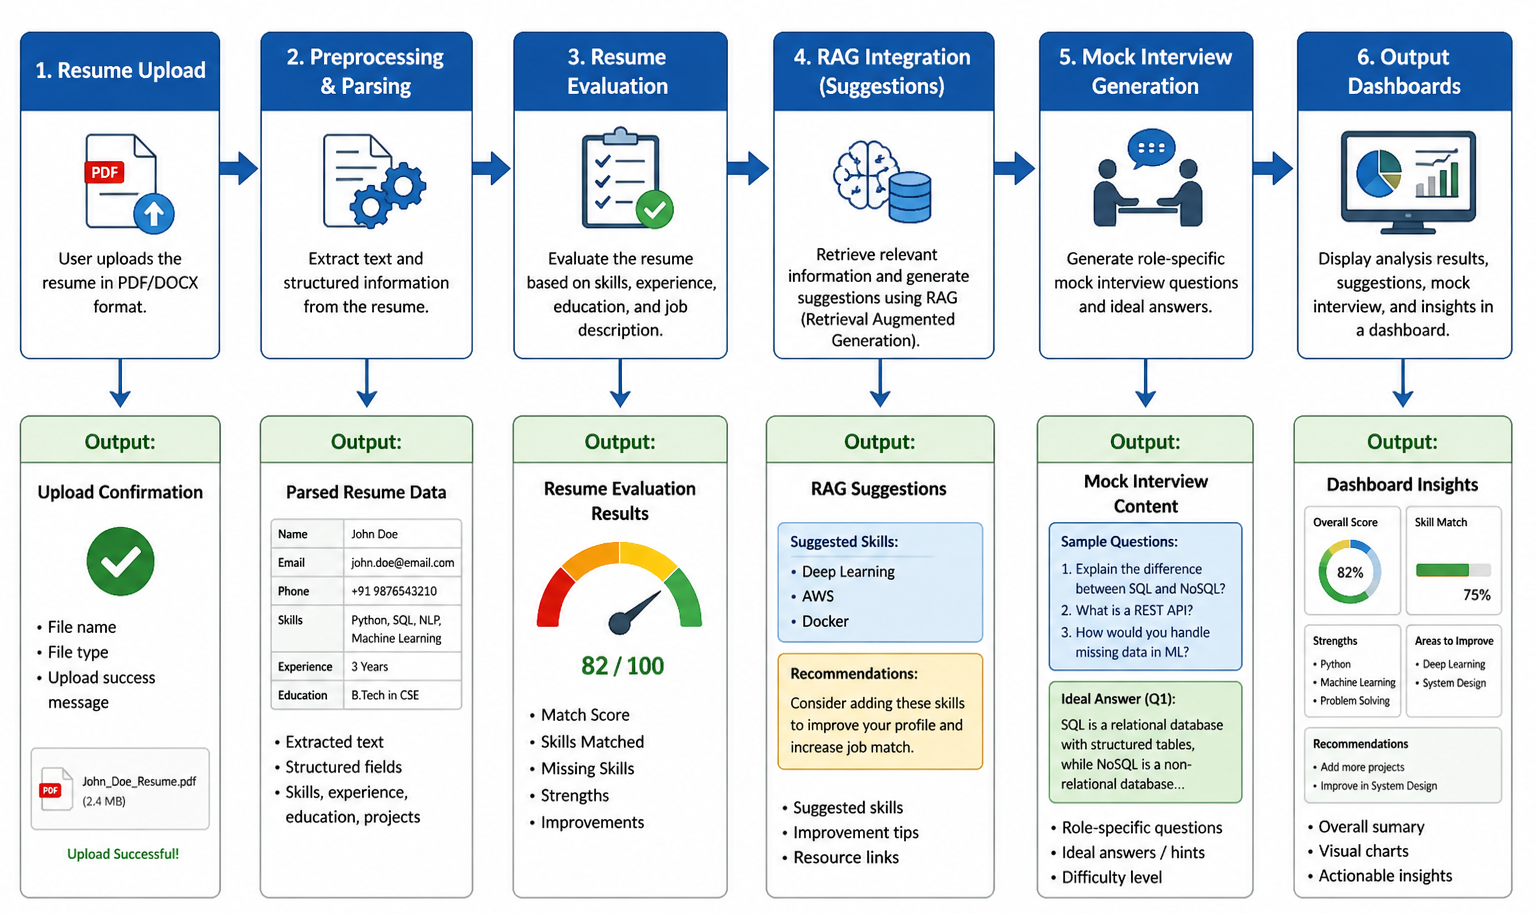
\includegraphics[width=1.0\textwidth]{images/Proposed system7.png}
 \captionof{figure}{Proposed system}
\end{figure}

\vspace{6pt}
{%\noindent
In addition, the system integrates semantic similarity models that analyze the meaning of both resumes and job descriptions rather than relying solely on keywords. This ensures that candidates with relevant skills are identified even if different wording is used.}


\vspace{6pt}
{%\noindent
The proposed system also includes a feedback and explanation module, which provides insights into why a resume matches or does not match a job. This improves transparency and helps candidates enhance their resumes.}


\section{Software Tools and Modules Used}
\vspace{6pt}
{%\noindent
The system uses NLP libraries such as spaCy and NLTK for text processing and entity extraction. These tools help in identifying important components like skills, organizations, and qualifications from resumes.}


\vspace{6pt}
{%\noindent
Machine learning and deep learning models such as BERT and other transformer-based architectures are used for semantic understanding and similarity matching. These models improve accuracy by capturing contextual meaning.}

\vspace{6pt}
{%\noindent
The backend of the system can be developed using Python frameworks, while the frontend can use technologies like React.js for user interaction. Databases are used to store resumes, job descriptions, and analysis results.}
\begin{figure}[ht]
\centering
 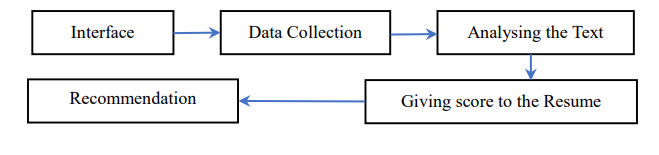
\includegraphics[width=1.0\textwidth]{images/Module Diagram.png}
 \captionof{figure}{Module Diagram}
\end{figure}


\vspace{6pt}
{%\noindent
The system is divided into multiple modules, including Resume Parser, NER Module, ATS Scoring Module, Semantic Matching Module, and Feedback Generation Module. Each module works together to provide a complete resume analysis solution.}

\noindent \textbf{1. Named Entity Recognition}
\begin{itemize}
    \item  Named Entity Recognition (NER) is an NLP technique used to identify and classify important information from unstructured text.
    \item It detects entities such as name, skills, education, experience organization, and dates from resumes.
    \item NER converts raw resume text into structured data, which can be easily analyzed by the system.
    \item After extracting entities, the system compares resume entities with job requirements.
    \item Each important entity is assigned a weight (points) based on its importance.
            \noindent Skills → High weight,
            \noindent Experience → Medium weight,
            \noindent Education \& Certifications → Lower weight
    \item Points are given when resume entities match job-required entities.
    \item The total points contribute to the overall ATS score
\end{itemize}
\vspace{6pt}
\noindent \textbf{2. ATS \& RAG Modules}
\begin{itemize}
    \item Applicant Tracking System (ATS) is used to evaluate and rank resumes based on job requirements.
    \item It compares extracted resume data with the job description using NLP techniques.
    \item ATS generates a match score that indicates how suitable a resume is for a particular role.
    \item Retrieval-Augmented Generation (RAG) is an advanced NLP technique     that combines information retrieval with text generation.
    \item Instead of generating answers only from a trained model, RAG first retrieves relevant data from an external knowledge source.
    \item Using the retrieved information, the system then generates accurate and context-aware responses
\end{itemize}
\noindent\textbf{3. Visual studio code :} 
Visual studio code is used as the development environment for implementing, training, and testing the resume analysis model. It provides an interactive environment with GPU support for faster training.


\section{Overall workflow}
The proposed methodology aims to design and implement an intelligent, automated re-cruitment system that leverages Machine Learning (ML) and Natural Language Processing(NLP) techniques to streamline the resume screening process. In this system, we utilizevarious NLP models to effectively process and analyze textual data present in resumes andjob descriptions. The system is developed to efficiently handle large volumes of resumes,extract meaningful insights, evaluate candidate suitability, and generate personalized mockinterview questions for shortlisted candidates. By incorporating NLP models for tasks suchas text preprocessing, feature extraction, and semantic analysis, the system improves the ac-curacy of candidate-job matching and overall decision-making. This methodology ensures
accuracy, scalability, and efficiency while reducing manual effort and improving hiring
quality.

{%\noindent 
The proposed methodology aims to design and implement an intelligent, automated recruitment system that leverages Machine Learning (ML) and Natural Language Processing (NLP) techniques to streamline the resume screening process. In this system, we utilize various NLP models to effectively process and analyze textual data present in resumes and job descriptions. The system is developed to efficiently handle large volumes of resumes, extract meaningful insights, evaluate candidate suitability, and generate personalized mock interview questions for shortlisted candidates. By incorporating NLP models for tasks such as text preprocessing, feature extraction, and semantic analysis, the system improves the accuracy of candidate-job matching and overall decision-making. This methodology ensures accuracy, scalability, and efficiency while reducing manual effort and improving hiring quality.}


The proposed system follows a structured and systematic workflow to automate the resume screening process and generate personalized mock interview questions. The workflow is designed as a multi-stage pipeline that transforms raw resume data into meaningful outputs, enabling efficient and accurate candidate selection. Each stage of the system performs a specific function, ensuring smooth data flow and effective processing.

\begin{itemize}
    \item \textbf{Resume and Job Description Input:}
    The workflow begins with the input stage, where resumes are collected from candidates in various formats such as PDF, Word documents, or text files. Along with this, recruiters provide job descriptions that specify the required skills, qualifications, and experience. These inputs act as the foundation for the entire process.
    \item \textbf{Data Extraction and Resume Parsing:} 
    In this stage, the system extracts relevant information from the resumes using NLP techniques. The unstructured resume data is converted into structured format by identifying key entities such as skills, education, experience, certifications, and contact details. This step ensures that important information is organized for further analysis.
    \item \textbf{Text Preprocessing:}
    The extracted text undergoes preprocessing to clean and standardize the data. This includes removing stop words, converting text to lowercase, eliminating special characters, and performing stemming or lemmatization. Preprocessing improves data quality and prepares it for feature extraction.
    \item \textbf{Feature Extraction:}
    The cleaned text is transformed into numerical representations using NLP models and techniques such as TF-IDF, Bag of Words, or word embeddings. This step allows machine learning models to understand and process the textual information effectively.
    \item \textbf{Candidate-Job Matching:}
    The system compares the features extracted from resumes with those from job descriptions. Similarity measures are used to evaluate how well each candidate matches the job requirements based on skills, experience, and keywords.
     \item \textbf{Candidate Scoring and Ranking:}
     Based on the matching results, each candidate is assigned a score. Candidates are then ranked in descending order according to their relevance and suitability for the job role. This helps recruiters focus on top candidates.
     \item \textbf{Shortlisting of Candidates:}
    Candidates who meet the required threshold are shortlisted for the next stage. This step filters out less relevant candidates and ensures that only qualified applicants proceed further.
    \item \textbf{Mock Interview Question Generation:}
    For shortlisted candidates, the system generates personalized mock interview questions. These questions are created based on the candidate’s skills, experience, and job role. The questions are categorized into technical, behavioral, and HR questions to provide comprehensive interview preparation.
    \item \textbf{Output Generation:}
    The final output includes:

\item Ranked list of candidates
\item Candidate scores and highlights
\item Generated mock interview questions

This information is presented to recruiters in a clear and structured format.
\item \textbf{User Interface and Interaction:}
    The system provides a user-friendly interface where recruiters can upload resumes, input job descriptions, and view results. This ensures ease of use and efficient interaction with the system.

    The overall workflow of the proposed system ensures a seamless and efficient recruitment process by integrating NLP and Machine Learning techniques. It automates resume analysis, improves candidate selection accuracy, and enhances interview preparation, making it a complete and intelligent recruitment solution.
    
\begin{figure}[ht]
\centering
 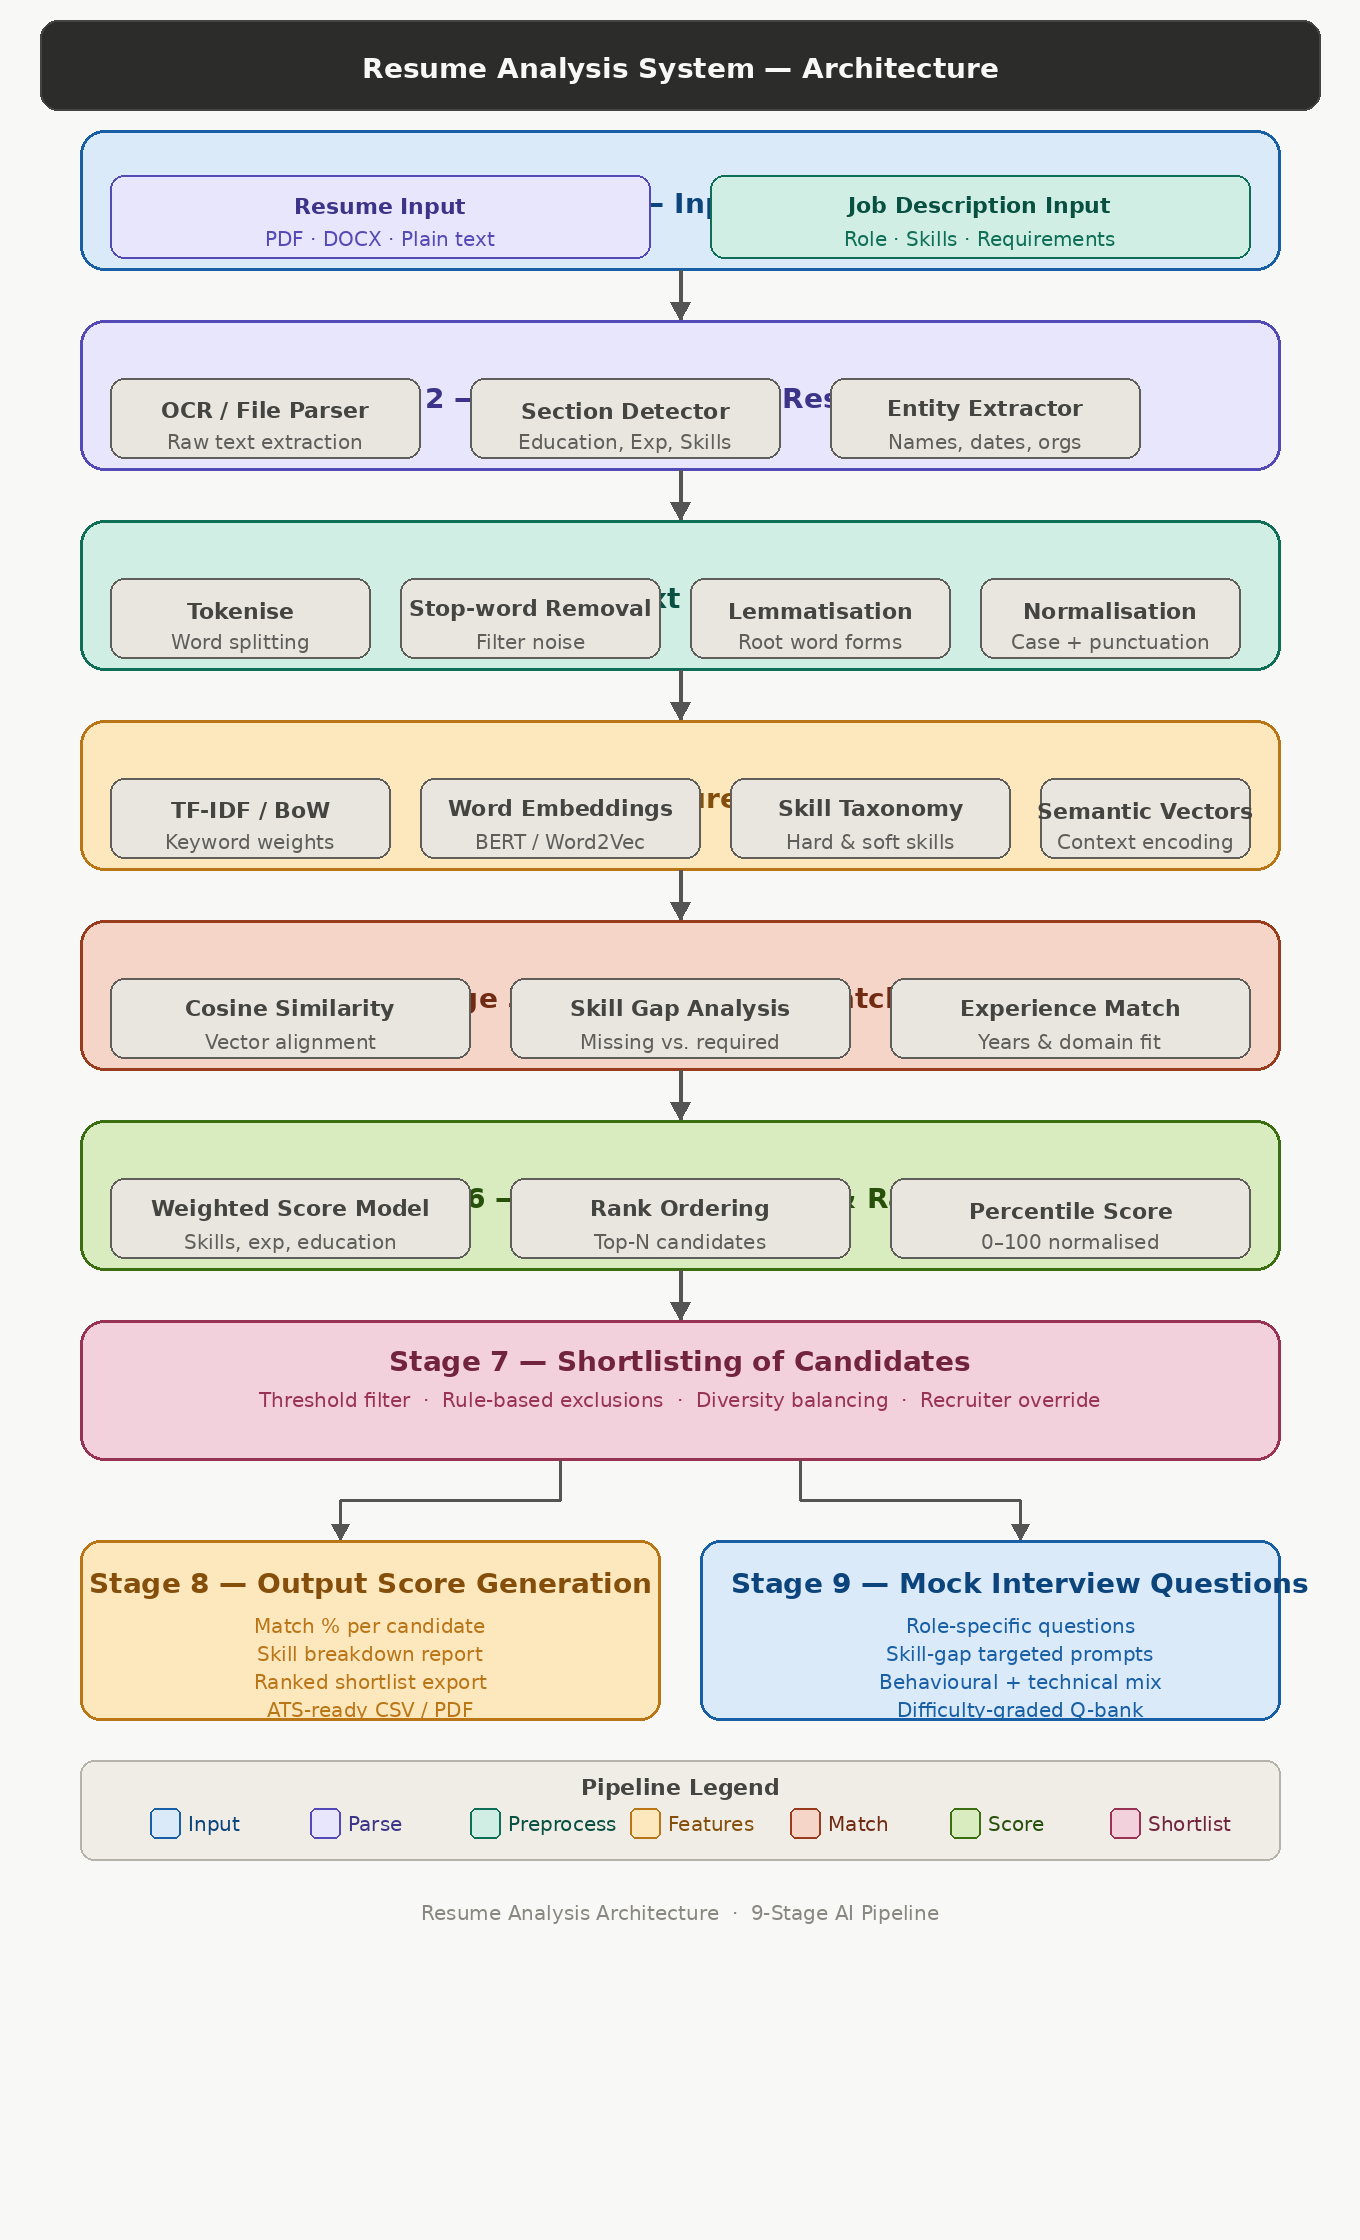
\includegraphics[width=0.8\textwidth]{images/workflow.png}
 \captionof{figure}{Workflow}
\end{figure}
    
\end{itemize}

